\documentclass[a4paper]{article}

% packages
\usepackage[utf8]{inputenc}
\usepackage[dutch]{babel}
\usepackage{hyperref}
\usepackage{graphicx}
\usepackage{listings}
\usepackage[toc]{glossaries}


% bibliografische databank
\usepackage[backend=biber, style=apa]{biblatex}
\DeclareLanguageMapping{dutch}{dutch-apa}
\addbibresource{stageverslag-2122.bib}


\makeglossaries
%%=============================================================================
%% Verklarende woordenlijst
%%=============================================================================
\newglossaryentry{kwartier}
{
    name=kwartier,
    description={Tijdelijke verblijfplaats voor militairen~\autocite{Wikipedia2021}},
    plural=kwartieren
}
\newglossaryentry{ccvc}
{
    name={CC V\&C},
    description={Competentie centrum Vliegend materieel \& Communicatie- en informatie-systemen}
}
\newglossaryentry{its}
{
    name=IT\&S,
    description={Information Technology \& Services}
}
\newglossaryentry{eenheid}
{
    name=eenheid,
    description={Een militaire eenheid bestaat uit een commando- en staf-element, uit uitvoerende militaire eenheden van een lager niveau en steuneenheden. Een militaire eenheid staat onder commando van een (onder)officier van voldoende rang~\autocite{Wikipedia2021a}},
    plural=eenheden
}
\newglossaryentry{lvm}
{
    name=LVM,
    description={Linux Volume Manager}
}
\newglossaryentry{rdp}
{
    name=RDP,
    description={Remote desktop protocol}
}
\newglossaryentry{acl}
{
    name=ACL,
    description={Access control list},
    plural={ACL's}
}
\newglossaryentry{selinux}
{
    name=SELinux,
    description={Security Enhanced Linux}
}
\newglossaryentry{db}
{
    name=db,
    description={Database},
    plural=db's
}

% Metadata
\title{Stageverslag}
\author{Pieter {Van Keer}}
\date{2021 - 2022}

\begin{document}
    
    % inhoudstafel
    \tableofcontents
    \pagebreak
    
    % kern
    %%=============================================================================
%% Voorwoord
%%=============================================================================
\section{Voorwoord}
\label{sec:voorwoord}

%% TODO:
%% Het voorwoord is het enige deel van de bachelorproef waar je vanuit je
%% eigen standpunt (``ik-vorm'') mag schrijven. Je kan hier bv. motiveren
%% waarom jij het onderwerp wil bespreken.
%% Vergeet ook niet te bedanken wie je geholpen/gesteund/... heeft



Dit stageverslag werd geschreven in het kader van de stage die ik liep bij Defensie van 21/02/2022 tot 27/05/2022. Dit was een zeer interessante periode omdat ik hier veel bijgeleerd heb.

Zoals vele andere dingen in het leven, kon ik dit niet alleen en daarom wil ik graag een aantal mensen bedanken. Steven beeckman, bedankt om mij zo goed te ontvangen bij Defensie, ook voor de vragen die ik had voor zowel de stage als bachelorproef kon ik steeds bij jou terecht. Tom De Leeuw, mijn stagementor, bedankt om mij te begeleiden en te helpen doorheen mijn stage. Wim De bruyn, mijn stagebegeleider, bedankt voor de opbouwende feedback en begeleiding tijdens de stage. Tot slot, Britt, die mij ondertussen al 3 jaar aanzet om het beste uit mezelf te halen.

\begin{flushleft}
    
Ik wens u veel leesplezier.
\end{flushleft}

\begin{flushleft}

Pieter Van Keer

Dendermonde, 27 mei, 2022

\end{flushleft}
    %%=============================================================================
%% Defensie
%%=============================================================================
%% stel stageplaats voor en schets waar je stage hebt gelopen.

\section{Defensie}
\label{sec:defensie}
%bron: https://www.mil.be/nl/over-defensie/#onze-organisatie
Defensie telt 26.179 personeelsleden, verdeeld over vier componenten: Landcomponent, Luchtcomponent, Marine en Medische Component. Daarnaast werken ze ook op de verschillende algemene directies en stafdepartementen, onder leiding van de Chef Defensie: admiraal Michel Hofman. Zie figuur~\ref{fig:organigram-defensie}

De personeelsleden van Defensie oefenen meer dan 300 verschillende beroepen uit. Dat maakt van Defensie een van de meest diverse werkgevers in het land, met zowel Nederlandstalige (54 \%) als Franstalige (46 \%) profielen. Militairen vormen de bulk van het personeelsbestand. Sommige functies vereisen echter geen uniform: bijna 6 \% ervan wordt ingevuld door burgerpersoneel. \autocite{Defensie2022}

\begin{figure}
    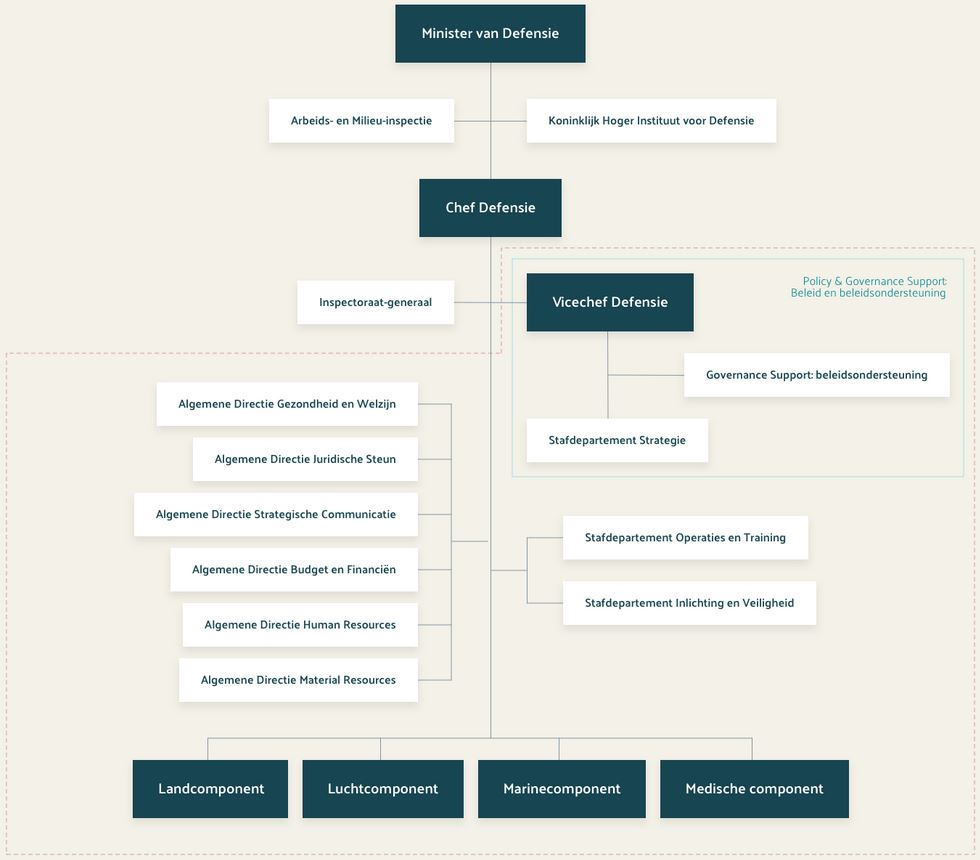
\includegraphics[width=\textwidth]{img/organigram-defensie.png}
    \caption{\label{fig:organigram-defensie}Organigram van Defensie~\autocite{Defensie2022}}
\end{figure}

\subsection{Stageplaats}

Defensie heeft verschillende \glspl{kwartier}, mijn stage vond plaats binnen de \gls{eenheid} \gls{ccvc} op het \gls{kwartier} Majoor Housiau gelegen te Peutie. Zie Figuur~\ref{fig:organigram-ccvc}

\begin{figure}
    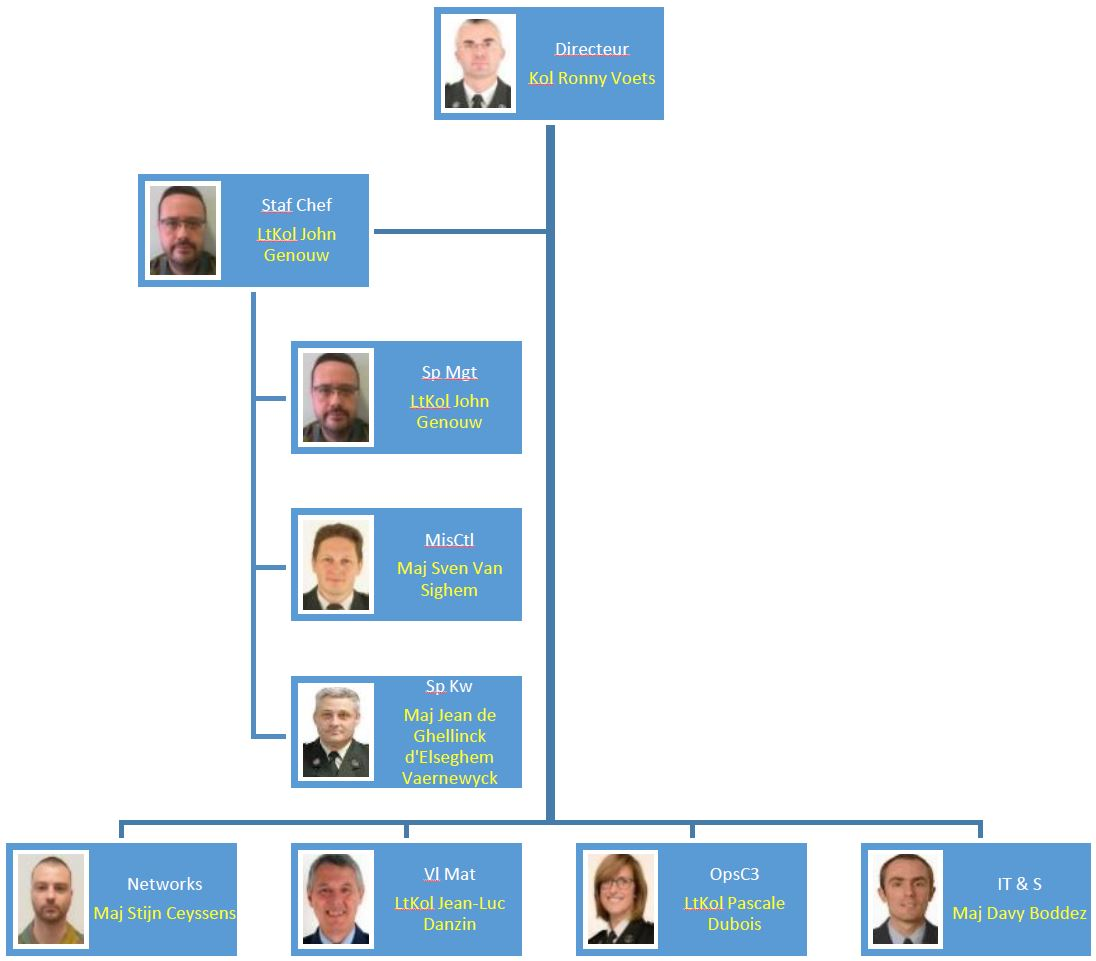
\includegraphics[width=\textwidth]{img/organigram-ccvc.png}
    \caption{\label{fig:organigram-ccvc}Organigram van de \gls{eenheid} \gls{ccvc}~\autocite{Defensie2022a}}
\end{figure}

Mijn stage was bij de afdeling Systems binnen het Departement \gls{its}. Zie figuur~\ref{fig:organigram-its}

\begin{figure}
    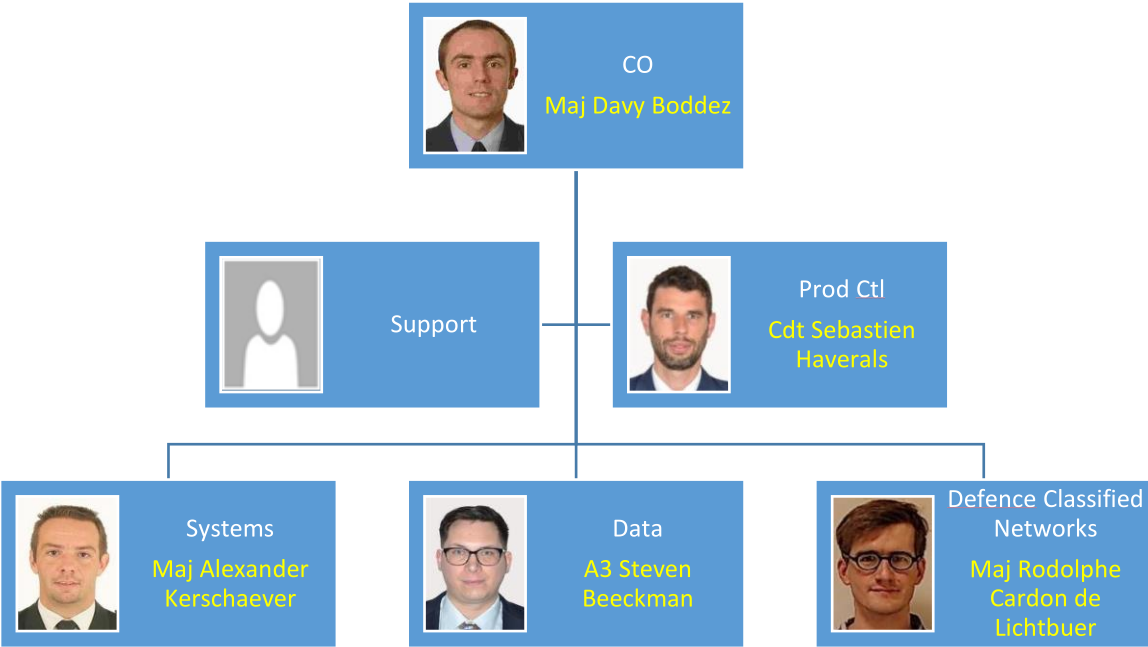
\includegraphics[width=\textwidth]{img/organigram-its.png}
    \caption{\label{fig:organigram-its}Organigram van het departement \gls{its}~\autocite{Defensie2022a}}
\end{figure}

Binnen de afdeling Systems zijn er 6 diensten:

\begin{itemize}
    \item linux
    \item windows
    \item oracle databanken
    \item Microsoft sql server
    \item prodctl
    \item techbu
\end{itemize}

Hoewel ik binnen elke dienst een introductie gekregen heb was miin stage vooral binnen de dienst linux.

Ik heb Defensie gekozen omdat ik ambitie heb om later bij Defensie te gaan werken. Op deze manier kan ik al eens kijken hoe het er aan toe gaat op de werkvloer.
    %%=============================================================================
%% Opdrachten
%%=============================================================================
% Opdracht template:

%\subsubsection{Beginsituatie}
%\subsubsection{Doel}
%\subsubsection{Plan van Aanpak}
%\subsubsection{Uitwerking}
%\subsubsection{Eindresultaat}
%\subsubsection{Business doelstellingen}
%\subsubsection{Persoonlijke doelstellingen}

\section{Opdrachten}
\label{sec:opdrachten}

\subsection{Backup-script moderniseren}

Binnen Defensie gebruikt men een bashscript genaamd ``bu\_script.sh'' om een backup te nemen van de databanken die bestaan op een machine en deze weg te schrijven op het netwerk.  
Ik kreeg de opdracht om dit script te moderniseren. Om de opdracht een beetje te vereenvoudigen moest ik de backup's lokaal wegschrijven.

\subsubsection{Beginsituatie}

Het script bestaat maar het is verouderd. Met het script is het mogelijk om meerdere instances van Mariadb/mysql te backuppen. Het script is zeer lang en moeilijk leesbaar.

\subsubsection{Doel}

\begin{itemize}
    \item moderniseer het script
    \item maak het script meer flexibel door gebruik te maken van meer variabelen
    \item genereer een rapport van de uitvoering van het script
    \item schrijf de backup lokaal weg onder de map ``$\sim$/backup''
\end{itemize}

\subsubsection{Plan van Aanpak}

\begin{enumerate}
    \item lees het script door en probeer de denkwijze te begrijpen van de persoon die het script geschreven heeft
    \item verwijder delen die niet meer van toepassing zijn
    \item voeg meer commentaar toe aan het script zodat iemand die het script later zal doornemen sneller weet wat er gebeurd
    \item gebruik meer functies aan zodat het script meer leesbaar wordt
    \item test het script
\end{enumerate}

\subsubsection{Uitwerking}

Ik ben begonnen met het script door te nemen en de logica proberen te verstaan. Tijdens dat ik dit deed heb ik extra commentaar geschreven om duidelijk te maken wat er juist gebeurde in het script. Na een kort gesprek met Tom hebben we besloten om het script enkel te beperken voor server die maar 1 instance hebben van mariadb/mysql. Hierdoor werd het script al veel meer leesbaar. Door extra hulpfuncties toe te voegen is de leesbaarheid ook verbeterd. Tijdens het testen heb ik er nog enkele bugs uitgehaald maar het script werkt zoals gevraagd.

\subsubsection{Eindresultaat}

Het eindresultaat is een script dat makkelijker te lezen/verstaan en flexibel is. Het script gaat een rapport genereren van de uitvoering en de backup was te vinden in de map ``$\sim$/backup''. Er is mogelijkheid om in te toekomst het script uit te breiden zodat dit een melding gaat genereren in Zabbix (monitoring tool).

\subsubsection{Business doelstellingen}

Voor de business was het belangrijk dat het script een moderne update kreeg. Dit was zeker het geval.

\subsubsection{Persoonlijke doelstellingen}

Voor mij persoonlijk was dit een geslaagde opdracht. Het script is nu meer flexibel en dit zal er voor zorgen dat men dit in de toekomst nog kan uitbreiden.


\subsection{Procedure upgrade mariadb}

Tegen 2024 moeten alle dbserver binnen Defensie draaien op Mariadb 10.6 op RHEL 8. Om deze transitie rustig te laten verlopen is er nood aan een procedure die men kan volgen tijdens zo een upgrade van een machine.

\subsubsection{Beginsituatie}

De dbserver bij Defensie draaien op mariadb 5.5 op RHEL 7.

\subsubsection{Doel}

Schrijf een procedure die men kan volgen om een machine te upgraden naar Mariadb 10.6 op RHEL 8. De procedure moet aandacht schenken aan volgende punten:

\begin{itemize}
    \item het besturingssysteem van de nieuwe machine is Red Hat Enterprise Linux (RHEL) 8
    \item er gaat geen data verloren
    \item de juiste mensen inlichten dat er onderhoud zal doorgevoerd worden op hun dbserver
\end{itemize}

\subsubsection{Plan van Aanpak}

Voor deze opdracht zal ik iteratief werken:

\begin{itemize}
    \item de eerste iteratie zal ik op papier (in grote lijnen) schetsen wat er moet gebeuren
    \item de tweede iteratie zal ik dit in een word-document gieten en laten nalezen door Tom
    \item de derde en volgende iteratie(s) zal ik de procedure meer specifiek maken
\end{itemize}

\subsubsection{Uitwerking}
\subsubsection{Eindresultaat}
\subsubsection{Business doelstellingen}
\subsubsection{Persoonlijke doelstellingen}

\subsection{High availability bij databanken}


Onderzoek hoe men binnen defensie high availability implementeren? Als er een db faalt en niet beschikbaar is moet de applicatie zonder problemen verderwerken. Volgende punten moeten zeker vermeld zijn:

\begin{itemize}
    \item is er een licentie voor nodig?
    \item is de software ondersteund door Red Hat?
    \item zijn er open source beperkingen?
    \begin{itemize}
        \item enkel voor commercieel gebruik?
        \item beperking voor militaire doeleinden?
    \end{itemize}
\end{itemize}

\subsubsection{Beginsituatie}

Binnen Defensie is er momenteel maar 1 databank achter een bepaalde applicatie. Dit zorgt er natuurlijk voor dat als die databank faalt, de applicatie ook niet meer zal werken.

\subsubsection{Doel}

Zorg ervoor dat er meerdere databanken met dezelfde data achter een bepaalde applicatie zitten.

\subsubsection{Plan van Aanpak}

Voor deze opdracht zal ik iteratief werken:

\begin{itemize}
    \item de eerste iteratie zal ik op papier (in grote lijnen) schetsen wat er moet gebeuren alsook ideeën opschrijven van productie die men mogelijk kan gebruiken
    \item de tweede iteratie zal ik dit in een word-document gieten en laten nalezen door Tom
    \item de derde en volgende iteratie(s) zal ik de procedure meer specifiek maken en uitbreiden
\end{itemize}

Nadat het document volledig is ga ik een handleiding maken om dit te implementeren en een eenvoudige opstelling testen met 2 servers.

\subsubsection{Uitwerking}
\subsubsection{Eindresultaat}
\subsubsection{Business doelstellingen}
\subsubsection{Persoonlijke doelstellingen}

\subsection{MS SQL logins}

\subsubsection{Beginsituatie}

De Jboss Application servers connecteren zich met MSSQL server met SQL logins en dus via SQL server authentication.

\subsubsection{Doel}

Voer een onderzoek en beantwoord volgende vragen:

\begin{itemize}
    \item Kan Windows authentication gebruikt worden?
    \item Wat zijn mogelijke alternatieven voor Authenticatie?
    \begin{itemize}
        \item Wat zijn voor- en nadelen (vooral op vlak van Security en Management)?
    \end{itemize}
    \item Welke configuratie/software/drivers moet er geïnstalleerd worden om dit mogelijk te maken?
\end{itemize}

\subsubsection{Plan van Aanpak}

Ik ga beginnen met mezelf bekend te maken met het onderwerp. Ik ga een virtuele machine vragen waar ik op kan testen. Daarna zal ik een oplossing proberen zoeken op het probleem, en als laatste zal ik deze testen.

%\subsubsection{Uitwerking}
%\subsubsection{Eindresultaat}
\subsubsection{Business doelstellingen}

Door het gebruikt van windows authentication zal het systeem veiliger worden.

%\subsubsection{Persoonlijke doelstellingen}
    %%=============================================================================
%% Eindereflectie
%%=============================================================================
\section{Eindreflectie}
\label{sec:Eindreflectie}

\subsection{Voldoet de stage aan hetgeen ik verwacht had?}

Ja, ik ben terecht gekomen bij toffe mensen die me met open armen ontvangen hebben. Het was een unieke ervaring om te werken in een militaire sfeer.

\subsection{Overwelke opdracht ben ik het meest trots?}

De procedure om mariadb te upgraden, daar ben ik het meest trots op. Ik heb een script geschreven in Python terwijl ik redelijk weinig ervaring heb met Python. Ook heb ik hier veel bijgeleerd, qls je ook een upgrade van een besturingssysteem moet doen dan is de upgrade minder vanzelfsprekend 

\subsection{Is dit het toekomstbeeld dat ik voor ogen heb?}

Ja, werken met linuxservers zie ik me in de toekomst zeker nog doen maar ik denk dat er ook andere dingen zijn die ik eens wil proberen zoals bijvoorbeeld \gls{ci}/\gls{cd} voorzien in een DevOps project.

\subsection{Vind je van jezelf dat je genoeg ervaring hebt opgedaan om nu in het werkveld te stappen?}

Zeker en vast, Ik heb veel bijgeleerd over linuxservers en het beheer ervan. Ook de provisioning van de server begrijp ik nu beter. Uiteraard als je bij een andere werkgever toekomst zal je sowieso even moeten aanpassen aan de manier van werken vooraleer je het beste uit jezelf kan halen.
    \pagebreak
    
    \appendix
    %%=============================================================================
%% Stage-logboek
%%=============================================================================

\section{Stagedagboek}
\label{sec:stagedagboek}

\subsection{Week 1}

\subsubsection{Maandag 21/02/2022}

\emph{Eerste stagedag}. Kennismaking met \textbf{Tom De Leeuw}, Tom
staat in voor het linuxgedeelte. Laptop ontvangen, vooral gepraat over mogelijkheden van de stage.

Werkwijze voor telewerken:

\begin{enumerate}
    \item Surf naar \url{https://portal.connect.mil.be} en meld aan met \textbf{itsme}
    \item Kies voor vpn. Eens de verbinding opstaat kan je beginnen met skype.
\end{enumerate}

\subsubsection{Dinsdag 22/02/2022}

werkuren: \emph{8:00 - 16:00}

Zelfstandig research gedaan naar \gls{lvm}. \url{https://access.redhat.com/documentation/en-us/red_hat_enterprise_linux/8/html/configuring_and_managing_logical_volumes/index}

Na de research enkele kleine opdrachtjes uitgevoerd op mijn eigen devserver binnen Defensie:

\begin{enumerate}
    \item aanmaken logical volume
    \begin{itemize}
        \item maak logical volume aan van 300mb
        \item mount logical volume op \texttt{/var/data01}
        \item herstart server en kijk of het nog bestaat.
    \end{itemize}
    \item aanpassen logical volume
    \begin{itemize}
        \item vergroot logical volume
        \item verklein logical volume
    \end{itemize}
    \item volume groups
    \begin{itemize}
        \item maak 2 volume groups van 100-200mb
    \end{itemize}
\end{enumerate}

Achteraf als afsluiter van de dag moest ik een grafische omgeving installeren op mijn devserver en proberen om via windows \gls{rdp} de server te kunnen overnemen.

\subsubsection{Woensdag 23/02/2022}

werkuren: \emph{8:00 - 16:00}

Zelfstandig research gedaan naar
\href{https://www.redhat.com/en/technologies/management/satellite}{Redhat
    Satellite}, \href{https://theforeman.org}{Foreman} en
\href{https://www.theforeman.org/plugins/katello/}{Katello}. Ook naar
filesecurity: \glspl{acl}, \gls{selinux}.

Verworven kennis toegepast in demo-omgeving. Samen met Tom de Satellite
omgeving ontdekt. Uitleg gekregen hoe alles werkt.

\subsubsection{Donderdag 24/02/2022}

werkuren: \emph{8:00 - 16:00}

Kennis opgefrist ivm Mariadb, mysql en appstreams in RHEL. Manueel
mariadb geïnstalleerd op devmachine, \gls{db} en users aangemaakt. Research
over puppet en aan de hand van puppet mariadb proberen installeren en
users en \glspl{db} aan te maken. Meeting bijgewoond met externe mensen.

\subsection{Week 2}

\subsubsection{Maandag 28/02/2022}

werkuren: \emph{08:00-16:00}

Afgewerkt waar ik vorige donderdag mee bezig was. Bezig aan het
moderniseren van het script \texttt{bu\_script.sh}.

\subsubsection{Dinsdag 01/03/2022}

werkuren: \emph{8:00 - 16:00}

\texttt{bu\_script.sh} afgewerkt. Eenvoudige zelfgeschreven versie.\\
Begin aan voorbereiding theorie voor donderdag.

\subsubsection{Woensdag 02/03/2022}

werkuren: \emph{8:00 - 16:00}

Voorbereiding voor Donderdag

\begin{itemize}
    \item research gedaan in verband met \href{https://www.zabbix.com/documentation/5.0/en/manual/introduction/about}{Zabbix} (monitoring tool)
    \item git kennis opgefrist
    \item toegang gekregen tot de gitlab servers van Defensie.
    \item hello world project geschreven in Puppet op mijn dev machine
\end{itemize}

\subsubsection{Donderdag 03/03/2022}

werkuren: \emph{8:00 - 16:00}

Introductie tot Zabbix en puppet door Donovan. Daarna zelf via puppet
zabbix proberen installeren op devmachine.

\subsection{Week 3}

\subsubsection{Maandag 07/03/2022}

werkuren: \emph{08:00-16:00}

\begin{itemize}
    \item denk oefening:    
    \begin{itemize}
        \item hoe kan je het \texttt{bu\_script.sh} uitbreiden zodat er een melding komt in Zabbix wanneer een backup faalt?
        \item zoek uit wat er misgegaan is met de devmachine (te weinig geheugen).
    \end{itemize}
\end{itemize}

\subsubsection{Dinsdag 08/03/2022}

werkuren: \emph{8:00 - 16:00}

Introductie in Jboss applicatie servers door Christophe. Christophe
heeft me alles goed uitgelegd en we hebben een testapplicatie gedeployed
op mijn devmachine. Ik heb (onder begeleiding van Christophe) een
applicatie mogen vernieuwen in de acceptatieomgeving. (netmanto)

\subsubsection{Woensdag 09/03/2022}

werkuren: \emph{8:00 - 16:00}

De introductie in Jboss Applicatie servers verder gezet en afgewerkt. We
hebben nu niet alles maar redelijk veel overlopen van jboss servers. Ook
is het nu duidelijk hoe deze gemonitord worden (Jboss Operations
Networks).

Een eerste stagegesprek.

\subsubsection{Donderdag 10/03/2022}

Werkuren: \emph{08:30 - 16:30}

Werkdag in Peutie.

De opdracht gekregen om een oplossing te zoeken voor volgende problemen:

\begin{itemize}
    \item hoe high availability implementeren voor een db die aan een applicatie hangt?
    \item maak een procedure om Mariadb 5.5 op RHEL 7.x to upgraden naar Mariadb 10.6 op RHEL 8 zonder verlies van gegevens.
\end{itemize}

Ook de toegangsbadge in orde gemaakt samen met Donovan.

\subsection{Week 4}

\subsubsection{Maandag 14/03/2022}

werkuren: \emph{08:00-16:00}

Verder gewerkt aan de denkoefeningen op een iteratieve manier. Alles
mooi in een word-documentje gegoten.

\subsubsection{Dinsdag 15/03/2022}

werkuren: \emph{8:00 - 16:00}

Verder gewerkt aan de denkoefeningen op een iteratieve manier. Er is
nood aan validatie van gebruikers en databanken. Hiervoor een concept
bedacht.

\subsubsection{Woensdag 16/03/2022}

werkuren: \emph{8:00 - 16:00}

Verder gewerkt aan de denkoefeningen.

Upgrade mariadb:

\begin{itemize}
    \item validatie voor users bedacht. gestart aan een script om dit uit te
    voeren maar ik zat vast gaandeweg dus nu ga ik eens kijken dat er geen
    andere manier is om dit te doen.
\end{itemize}

db high availability:

\begin{itemize}
    \item iteratie afgewerkt. Nu wachten op feedback.
\end{itemize}

Stageverslag: structuur opgemaakt.

\subsubsection{Donderdag 17/03/2022}

Werkuren: \emph{08:15 - 16:15}

Fysiek in Peutie.

Normaal was er een introductie van \gls{mssql} gepland vandaag maar deze is
verzet naar een later moment. Ter vervanging heb ik verschillende
praktische oefeningen gedaan ivm \gls{lvm} op mijn devmachine. Ook dit
allemaal besproken met Tom.

\subsection{Week 5}

\subsubsection{Maandag 21/03/2022}

werkuren: \emph{08:00-16:00}

Verder gewerkt aan de denkoefening om high availability te implementeren
bij databanken. Tom heeft voor mij een aantal virtuele machines laten
maken zodat ik hierop kan testen.

Stageverslag verder aangevuld.

\subsubsection{Dinsdag 22/03/2022}

Geen stage.\\
Jobevent van HoGent


\subsubsection{Woensdag 23/03/2022}

werkuren: \emph{8:00 - 16:00}

Verder gewerkt aan de denkoefening om high availability te implementeren
bij databanken: Testopstelling gemaakt.

\begin{itemize}
    \item
    databank master
    \item
    databank slave
    \item
    reverse proxy
\end{itemize}

Zie Figuur \ref{fig:netwerkdiagram-db-replicatie}, Dit is het netwerkdiagram van de opstelling.

\begin{figure}
    \centering
    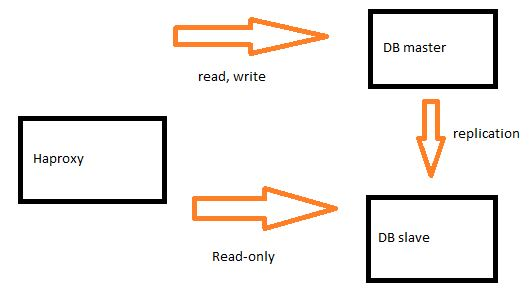
\includegraphics{img/networkdiagram_db_replication.JPG}
    \caption{\label{fig:netwerkdiagram-db-replicatie}netwerk diagram}
\end{figure}

Er is nog uitbreiding mogelijk: Hoe van replica een master maken?

\subsubsection{Donderdag 24/03/2022}

Fysiek in Peutie

werkuren: \emph{8:00 - 16:00}

Introductie van \emph{\gls{mssql}}\\
Onderzoeksopdracht besproken. ik zal hierover nog een document
ontvangen.\\
Tom heeft mij een rondleiding gegeven in de serverroom van in Peutie.

In de namiddag was er een drink binnen defensie waar de kolonel een
toespraak heeft gehouden. Het was tof om deze bij te wonen.

\subsection{Week 6}

\subsubsection{Maandag 28/03/2022}

werkuren: \emph{08:00-16:00}

Gewerkt aan de opdracht voor \gls{mssql}. Vooral research gedaan en mezelf
bekend gemaakt met het onderwerp. Ook een virtuele machine gevraagd om dingen te testen.


\subsubsection{Dinsdag 29/03/2022}

werkuren: \emph{08:00-16:00}

Bijlagen toegevoegd aan stageverslag. Verder onderzoek gedaan voor \gls{mssql}.
Gewacht op de virtuele machine.

Ad hoc een taak gekregen van Tom: schrijf een patch voor een databank. zie bijlage \ref{subsec:tables_patch}

\subsubsection{Woensdag 30/03/2022}

werkuren: \emph{08:00-16:00}

Blijkbaar is het niet simpel om voor mij een virtuele machine te voorzien dus we hebben het het opgelost door een named instance te maken op een bestaande server. Hierdoor heb ik enkele dingen kunnen testen in \gls{mssql}.

\subsubsection{Donderdag 31/03/2022}

werkuren: \emph{08:00-16:00}

Telewerken.

Verder gewerkt aan de opdracht van \gls{mssql}. Begonnen aan een script te schrijven voor de conversie van de logins/users te doen.  
Dit is moeilijker dan ik gedacht had.

\subsection{Week 7}

\subsubsection{Maandag 04/04/2022}

werkuren: \emph{08:00-16:00}

Verder gewerkt aan de opdracht van \gls{mssql}, niet gemakkelijk. Men kan zeggen dat ik vast zit.  
Johan was niet online dus ik kon hem niet bereiken om hulp te vragen.

\subsubsection{Dinsdag 05/04/2022}

werkuren: \emph{08:00-16:00}

Verder gewerkt aan de opdracht. Zit nog steeds vast, Johan niet online.

\subsubsection{Woensdag 06/04/2022}

werkuren: \emph{08:00-16:00}

Hulp gevraagd aan Johan maar nog geen antwoord gekregen. Voor de rest verder gewerkt aan de opdracht van \gls{mssql}.

\subsubsection{Donderdag 07/04/2022}

werkuren: \emph{08:00-16:00}

Telewerken.

Verder gewerkt aan \gls{mssql}.

\subsection{Week 8}

\subsubsection{Maandag 11/04/2022}

Afwezig

\subsubsection{Dinsdag 12/04/2022}

Afwezig

\subsubsection{Woensdag 13/04/2022}

Afwezig

\subsubsection{Donderdag 14/04/2022}

Afwezig

\subsection{Week 9}

\subsubsection{Maandag 19/04/2022}

geen stage. (paasmaandag)

\subsubsection{Dinsdag 20/04/2022}

werkuren: \emph{08:00-16:00}

Verder gewerkt aan de opdracht van \gls{mssql}. Ik zit hierin vast en ik heb nog geen contact kunnen maken met Johan. Tom had vandaag geen tijd om mij te helpen maar zal morgen contact opnemen met mij.

\subsubsection{Woensdag 21/04/2022}

werkuren: \emph{10:00-17:00}

Stand van zaken voor de opdracht van \gls{mssql} besproken met Tom. Johan heeft deze week nog verlof en zal vanaf volgende week terug aanwezig zijn. Contact gehad met Steven om een moment in te plannen om de mogelijkheden na de stage te bespreken.

\subsubsection{Donderdag 22/04/2022}

werkuren: \emph{08:00-16:00}

Begonnen aan het script om de users te checken voor de opdracht mysql migratie.

\subsection{Week 10}

\subsubsection{Maandag 25/04/2022}

werkuren: \emph{08:15-16:15}

Contact gehad met Johan en Donovan over de opdracht van \gls{mssql}. Meer info gezocht over de jtds driver. ook naar de jdbc driver gekeken.

\subsubsection{Dinsdag 26/04/2022}

werkuren: \emph{08:15-16:15}

Verder gewerkt aan de oefening van \gls{mssql}: meer info gezocht over de jtds en jdbc drivers. niet gevonden wat ik wou vinden.

Om mijn gedachten eens te verzetten heb ik nog eens gekeken naar het script `check\_users.py` en heb ik de output een aangepast zodat er nu een waarschuwing staat en verder gescrheven aan het stageverslag.

Voor de opdracht High availability voor mariadb: Research gedaan over hoe we in plaats van master-slave naar master-master kunnen gaan.


\subsubsection{Woensdag 27/04/2022}

werkuren: \emph{10:00-17:30}

Verder gezocht naar een oplossing voor de jtds driver. Steeds niet gevonden, morgen ga ik hierover met Donovan proberen praten om samen een oplossing te zoeken.
Nagedacht over hoe ik een testopstelling ga opzetten voor een master-master opstelling bij de opdracht High availability voor mariadb.
Stageverslag verder aangevuld.

\subsubsection{Donderdag 28/04/2022}

werkuren: \emph{8:15-16:15}

Fysiek in Peutie, JTDS driver:

\begin{itemize}
    \item Geen opzoekwerk mogelijk want binnen het netwerk van Defensie is het internet nog niet 100% opengesteld voor het personeel.
\end{itemize}

Opdracht High Availability voor mariadb:

\begin{itemize}
    \item Netwerkdiagram aangepast zodat dit een master-master oplossing is. Nog niet getest. 
\end{itemize}

Upgrade mariadb:

\begin{itemize}
    \item Nagedacht hoe we een script kunnen schrijven die de check voor de databases doet.
    \item Check\_users. Python show grants uitvoeren voor elke user. <https://codefather.tech/blog/shell-command-python/>
    \item Check\_users:
    \begin{itemize}
        \item verder gewerkt aan het script, logica gescrheven om grants uit te lezen rechtstreeks van de db.
        \item input veranderd dat het script de users ook rechtstreeks uit de db gaat halen.
    \end{itemize}
\end{itemize}


\subsection{Week 11}

\subsubsection{Maandag 02/05/2022}

werkuren: \emph{8:30-16:30}

Een moment afgesproken met Donovan waar hij een scripting opdracht zal uitleggen en waar ik enkele vragen kan stellen voor een lopende opdracht (mssql) en waar ik enkele vragen kan stellen ivm met mijn bachelorproef. Dit zal waarschijnlijk donderdag plaatsvinden in Peutie.

Verder gewerkt aan het check\_users script.

\subsubsection{Dinsdag 03/05/2022}

werkuren: \emph{8:30-16:30}

Frustrerende dag achter de rug. Verder gewerkt aan het check\_users script maar ik zit vast bij het vergelijken van de 2 puppet bestanden. Documentatie verder aangevuld.


\subsubsection{Woensdag 04/05/2022}

werkuren: \emph{8:15-16:15}

Check\_users script even op kant gelegd. Beginnen nadenken hoe ik het check\_database script zal schrijven. Stageverslag nog extra aangevuld.


\subsubsection{Donderdag 05/05/2022}

werkuren: \emph{8:00-16:00}

Fysiek in Peutie.

Samengezeten met Donovan omdat ik enkele vragen had voor hem ivm met een aantal opdrachten en ook over mijn bachelorproef.

Samen met Donovan en Steven nog een gesprek gehad om te praten over de bachelorproef. Steven gaat mij in contact brengen met personen die bij Smals werken om mij een beetje uitleg te geven hoe te daar te werk gaan.
Een moment afgesproken met Tom om mijn opdrachten eens te bekijken dit zal volgende donderdag plaatsvinden (12/05/2022)

check\_database:

\begin{itemize}
    \item research gedaan naar welke commando's ik moet gebruiken om de nodige data te verkrijgen uit de db.
    \item code geschreven voor file structuur op te zetten.
\end{itemize}

mssql:

\begin{itemize}
    \item alternatieve methodes gezocht.
\end{itemize}

\subsection{Week 12}

\subsubsection{Maandag 09/05/2022}

werkuren: \emph{8:15-16:15}

Aan stageverslag gewerkt. Verder opgezocht voor mssql

\subsubsection{Dinsdag 10/05/2022}

werkuren: \emph{8:15-16:15}

Enkele bugs uit de handleiding gehaald om replicatie te configureren.  
Status van de opdrachten toegevoegd in de readme

Aan het script \verb*|check_databases| gewerkt.

\subsubsection{Woensdag 11/05/2022}

Afwezig wegens een evenement van Telenet waar ik naartoe ben gegaan met toestemming van Tom.

\subsubsection{Donderdag 12/05/2022}

werkuren: \emph{8:00-16:00}

Fysiek in Peutie

Verder geschreven aan het \verb*|check_databases| script.

Samengezeten met Tom om mijn opdrachten eens te overlopen + enkele vragen gesteld over het \verb*|check_databases| script.

Een besluit beginnen schrijven voor de opdracht van mssql

\subsection{Week 13}

\subsubsection{Maandag 16/05/2022}

werkuren: \emph{8:00-16:00}

een manier gevonden om de titelpagina toe te voegen aan het stageverslag.

mssql:

\begin{itemize}
	\item conclusie geschreven voor de opdracht van mssql. Deze opdracht is nu ook afgerond.
	\item het stageverslag ook de opdracht mssql up-to-date gemaakt.
\end{itemize}

Mariadb replication:

\begin{itemize}
	\item master-master geprobeerd en gefinaliseerd.
	\item handleiding geupdate
	\item het stageverslag ook de opdracht Mariadb replication up-to-date gemaakt.
\end{itemize}

\subsubsection{Dinsdag 17/05/2022}

werkuren: \emph{8:30-16:30}

Nagedacht hoe ik verder moet met het check\_users script.

documentatie aangevuld.

\subsubsection{Woensdag 18/05/2022}

werkuren: \emph{8:00-16:00}

Verder gewerkt aan check\_users. Formaat gewijzigd voor de puppet config.

\subsubsection{Donderdag 19/05/2022}

werkuren: \emph{8:00-16:00}

Fysiek in Peutie.

Verder gewerkt aan check_users script, het enige wat nog moet gebeuren is puppet vergelijken. Nog steeds het probleem om puppet configuratie te gaan vergelijken.

\subsection{Week 14}

\subsubsection{Maandag 23/05/2022}

\subsubsection{Dinsdag 24/05/2022}

\subsubsection{Woensdag 25/05/2022}

\subsubsection{Donderdag 26/05/2022}

Hemelvaart
    \pagebreak
    %%=============================================================================
%% Install Mariadb Replication
%%=============================================================================

\section{MariaDB: Replication installation guide}

\subsection{Steps}

\subsubsection{Database replication}

\begin{enumerate}
    \item install MariaDB
    \item start and config MariaDB on primary server
    \item config master firewall
    \item start and config MariaDB on replica server
    \item test MariaDB
\end{enumerate}

\subsubsection{Reverse proxy}

\begin{enumerate}
    \item install proxy
    \item config proxy
    \item test proxy
\end{enumerate}

\subsection{Install MariaDB}

The repository is already there so we just have to install some packages.

\begin{lstlisting}
    sudo dnf install MariaDB-server MariaDB-backup
\end{lstlisting}

\subsection{Start/config primary server}

Edit config file with following:

\begin{lstlisting}
    [mariadb]
    log_bin
    server_id=1
    log-basename=master
    binlog-format=mixed
\end{lstlisting}

\textit{server\_id} is a unique value.\\
Start the dbserver:

\begin{quote}
    If already running, restart dbserver to apply config.
\end{quote}

\begin{lstlisting}
    systemctl enable mariadb --now
\end{lstlisting}

There should be at least 1 user created for replication:

Create user accounts:

\begin{quote}
    Each account should be created on the master so replication can make these accounts on the slaves.
\end{quote}

\subsubsection{Replication user}

\begin{lstlisting}
    CREATE USER 'repl'@'slave_ip' IDENTIFIED BY 'test';
\end{lstlisting}

Grant required privileges.

\begin{lstlisting}
    GRANT REPLICATION SLAVE
    ON *.* TO repl@'slave_ip';
\end{lstlisting}

\subsection{Start/config replica server}

\begin{lstlisting}
    [mariadb]
    log_bin
    server_id=2
    log-basename=master
    binlog-format=mixed
\end{lstlisting}

\textit{server\_id} is a unique value.\\

\begin{lstlisting}
    SHOW SLAVE STATUS;
    +--------------------+----------+--------------+------------------+
    | File               | Position | Binlog_Do_DB | Binlog_Ignore_DB |
    +--------------------+----------+--------------+------------------+
    | master1-bin.000096 |      568 |              |                  |
    +--------------------+----------+--------------+------------------+
\end{lstlisting}

Take notes of the filename and position

\begin{lstlisting}
    CHANGE MASTER TO
    MASTER_HOST='master_ip',
    MASTER_USER='replication_user',
    MASTER_PASSWORD='test',
    MASTER_PORT=3306,
    MASTER_LOG_FILE='master-bin.000096',
    MASTER_LOG_POS=568,
    MASTER_CONNECT_RETRY=10;
\end{lstlisting}

\begin{quote}
    With fresh master, you don't need to specify `MASTER\_LOG\_FILE` and `MASTER\_LOG\_POS`
\end{quote}

\subsubsection{Start replication}

\begin{lstlisting}
    START SLAVE;
    SHOW SLAVE STATUS;
\end{lstlisting}

If replication is running properly, both `Slave\_IO\_Running` and `Slave\_SQL\_Running` should be `Yes`.


\subsection{Test replication}

Use the following url to test replication: \url{https://mariadb.com/docs/deploy/topologies/primary-replica/enterprise-server-10-3/test-es/}

\subsection{Install proxy}

I chose to go with `haproxy`.\\
To install this proxy just use dnf.

\begin{lstlisting}
    sudo dnf install haproxy
\end{lstlisting}

\subsection{Config proxy}

\subsubsection{Edit configuration file}

\begin{lstlisting}
    # /etc/haproxy/haproxy.cfg
    
    defaults
    mode  tcp
    option mysql-check user haproxy_health
    frontend frontend
    # read-requests will arrive at port 3100
    bind *:3100
    # write-requests will arrive at port 3200
    bind *:3200
    # if write send to masters
    use_backend db_masters if { dst_port 3200 }
    # if read sent to slaves
    default_backend db_slaves
    
    backend db_masters
    server master1 10.8.131.120:3306
    
    backend db_slaves
    server slave1 10.8.131.121:3306
    server master1 10.8.131.120:3306
\end{lstlisting}

\subsubsection{(re)start service}

\begin{lstlisting}
    sudo systemctl enable haproxy --now
\end{lstlisting}

\subsubsection{SELinux}

\begin{lstlisting}
    setsebool haproxy_connect_any 1
\end{lstlisting}

\subsection{Test proxy}

To test proxy, use  port 3200 te write data and port 3100 to query data.
    
    % Verklarende woordenlijst
    \pagebreak
    \printglossary[title=Verklarende woordenlijst, toctitle=Verklarende woordenlijst]
    
    
    %Referentielijst
    \pagebreak
    \printbibliography[heading=bibintoc]
    
    
\end{document}